\capitulo{3}{Conceptos teóricos}

%En aquellos proyectos que necesiten para su comprensión y desarrollo de unos conceptos teóricos de una determinada materia o de un determinado dominio de conocimiento, debe existir un apartado que sintetice dichos conceptos.

Para la comprensión de este proyecto es necesaria la explicación de algunos conceptos teóricos que introduciré en este apartado. Para ello este apartado se ha organizado en seis bloques principales: fitolito, inteligencia artificial, procesamiento de imágenes, minería de datos, \textit{deep learning} y detección de objetos.

\section{Fitolito y su complejidad}

Los fitolitos son particulas microscópicas de silice de opalo producidas dentro y entre las celulas de muchas plantas. Además, son partículas muy resilientes y preservadas hasta la actualidad en forma de microfósiles. Estos son utilizados en la investigación de paleoambientes\footnote{Consistente en la reconstrucción de entornos antiguos.}, botánica, geología y arqueología~\cite{phytolith}.

Existen multitud de tipos de fitolitos, pero en este proyecto nos centramos en un conjunto de tipos más delimitado, según los requisitos de nuestros clientes. Los cuales se encuentran concrétamente interesados en el área de la arqueobotánica. En total trabajamos con 7 tipos de fitolitos:

\begin{itemize}
	\item Bilobate
	\item Bulliform
	\item Cyperaceae
	\item Rondel
	\item Saddle
	\item Spherical
	\item Trichomas
\end{itemize}

Como previamente comenté en la introducción del proyecto~\ref{intro}, en este proyecto nos enfrentamos con varias problemáticas. Una de ellas son los distintos tamaños y la tridimensionalidad de estos, lo cual introduce una gran variabilidad en sus apariencias. En la figura \ref{fig:3.1.1} observamos dos fotografías por cada uno de los tipos de fitolito que se encuentran en nuestro ámbito de estudio. Pudiendo observar en ella la variabilidad a la que hago referencia dentro de un mismo tipo de fitolito.

\begin{figure}
	\centering
	\begin{subfigure}[b]{0.2\textwidth}
        \includegraphics[width=\textwidth]{Bilobate/1}
        \caption{Bilobate 1}
    \end{subfigure}
    \begin{subfigure}[b]{0.2\textwidth}
        \includegraphics[width=\textwidth]{Bilobate/2}
        \caption{Bilobate 2}
    \end{subfigure}
    \begin{subfigure}[b]{0.2\textwidth}
        \includegraphics[width=\textwidth]{Bulliform/1}
        \caption{Bulliform 1}
    \end{subfigure}
    \begin{subfigure}[b]{0.2\textwidth}
        \includegraphics[width=\textwidth]{Bulliform/2}
        \caption{Bulliform 2}
	\end{subfigure}
    \begin{subfigure}[b]{0.2\textwidth}
        \includegraphics[width=\textwidth]{Cyperaceae/1}
        \caption{Cyperaceae 1}
    \end{subfigure}
    \begin{subfigure}[b]{0.2\textwidth}
        \includegraphics[width=\textwidth]{Cyperaceae/2}
        \caption{Cyperaceae 2}
    \end{subfigure}
    \begin{subfigure}[b]{0.2\textwidth}
        \includegraphics[width=\textwidth]{Rondel/1}
        \caption{Rondel 1}
    \end{subfigure}
    \begin{subfigure}[b]{0.2\textwidth}
        \includegraphics[width=\textwidth]{Rondel/2}
        \caption{Rondel 2}
    \end{subfigure}
    \begin{subfigure}[b]{0.2\textwidth}
        \includegraphics[width=\textwidth]{Saddle/1}
        \caption{Saddle 1}
    \end{subfigure}
    \begin{subfigure}[b]{0.2\textwidth}
        \includegraphics[width=\textwidth]{Saddle/2}
        \caption{Saddle 2}
    \end{subfigure}
    \begin{subfigure}[b]{0.2\textwidth}
        \includegraphics[width=\textwidth]{Spherical/1}
        \caption{Spherical 1}
    \end{subfigure}
    \begin{subfigure}[b]{0.2\textwidth}
        \includegraphics[width=\textwidth]{Spherical/2}
        \caption{Spherical 2}
    \end{subfigure}
    \begin{subfigure}[b]{0.2\textwidth}
        \includegraphics[width=\textwidth]{Trichomas/1}
        \caption{Trichomas 1}
    \end{subfigure}
    \begin{subfigure}[b]{0.2\textwidth}
        \includegraphics[width=\textwidth]{Trichomas/2}
        \caption{Trichomas 2}
    \end{subfigure}
    \caption[Conjunto de ejemplos de distintos tipos de fitolitos.]{Conjunto de ejemplos de distintos tipos de fitolitos. Las imágenes que aquí se presentan han sido obtenidas mediante el etiquetador de imágenes desarrollado en este proyecto.}
	\label{fig:3.1.1}
\end{figure}

Además, introduzco dos imágenes etiquetadas en la figura~\ref{fig:3.1.2}. Reflejando en ella la diferencia de tamaños entre los distintos tipos de fitolitos, a la que previamente hacía referencia. Lo cual aporta mayor complejidad al problema que estamos acometiendo. 

\begin{figure}
	\centering
	\begin{subfigure}[b]{0.8\textwidth}
        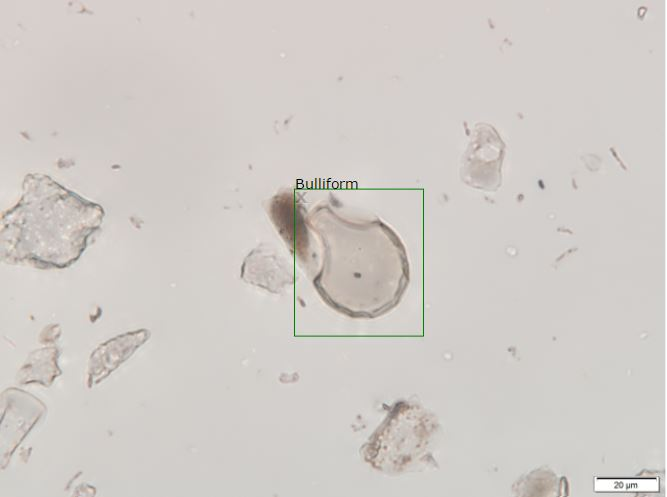
\includegraphics[width=\textwidth]{fitolito_ejemplo_1}
        \caption{Ejemplo bulliform etiquetado}
    \end{subfigure}
    \begin{subfigure}[b]{0.8\textwidth}
        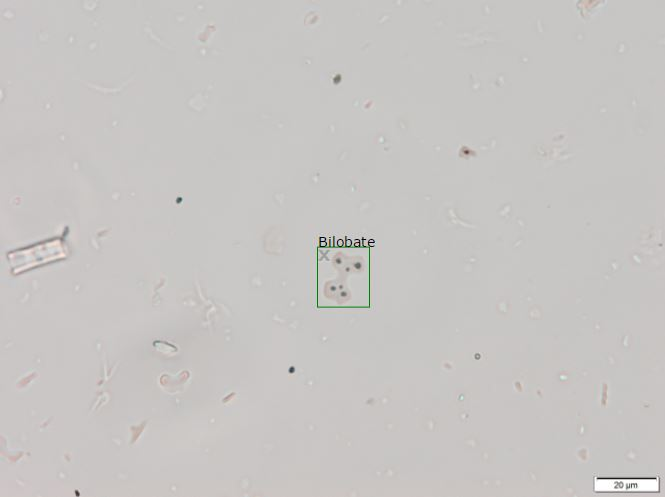
\includegraphics[width=\textwidth]{fitolito_ejemplo_2}
        \caption{Ejemplo bilobate etiquetado}
    \end{subfigure}
    \caption{Comparación de tamaño entre distintos tipos de fitolitos}
	\label{fig:3.1.2}
\end{figure}

Y, finalmente, destacar otra problemática que plantea este contexto. Las imágenes tienen un alto grado de ruido, ya que estas no solo contienen  fitolitos. Sino que contienen otras materias o restos sin relevancia alguna, como observamos en la figura~\ref{fig:3.1.3}.

\begin{figure}
\centering
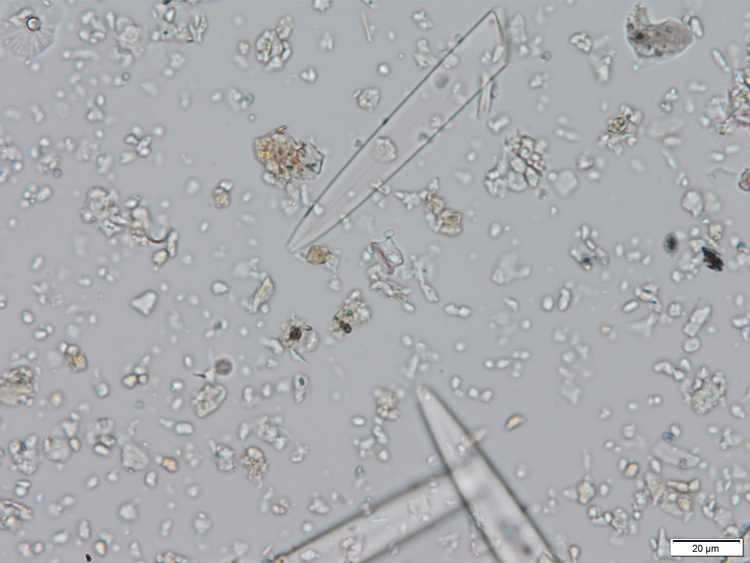
\includegraphics[width=0.8\textwidth]{fitolito_ruido}
\caption{Imagen con mucho ruido.}
\label{fig:3.1.3}
\end{figure}

\section{Inteligencia artificial}

Inteligencia artificial, que comúnmente aparece como las siglas IA o AI del inglés Artificial Intelligence, consiste en otorgar a las máquinas la capacidad de realizar acciones que habitualmente son realizadas por humanos, imitando la inteligencia cognitiva humana~\cite{alanturing:ai}. Esta podría ser una posible definición de Inteligencia artificial, pero existen multitud~\cite{russell1995modern}. Algunos posibles ejemplos conocidos por todos en los que se aplica la IA son el coche autónomo, videojuegos, asistentes personales, reconocimiento facial en imágenes, entre otros.

\subsection{Aprendizaje automático}

Apredizaje automático, o en inglés \textit{machine learning}, es un campo de la informática cuyo objetivo es dar a los computadores la capacidad de aprender sin explícitamente haber sido programados~\cite{wiki:machinelearning}. Además, se encarga de construir modelos para problemas en los que un algoritmo programado con un conjunto de instrucciones estáticas no puede conseguir buenos resultados o es muy complejo hacer que lo sean.



\subsubsection{Aprendizaje supervisado y no supervisado}

En esta sección vamos a distinguir entre aprendizaje supervisado y no supervisado, ambas técnicas pertenecientes al campo de \textit{machine learning}.

Aprendizaje supervisado es una técnica que consiste en la inferencia de una función partiendo de un conjunto de datos de entrenamiento etiquetado~\cite{wiki:supervisedLearning}. Dos de las tareas más comunes del aprendizaje supervisado son clasificación y regresión. Es decir, para tareas en las que el resultado deseado sea obtener una variable que nos informe a que clase pertenece una determinada instancia, lo cual es un valor discreto, o para tareas en las que se desea obtener un valor continuo. Dos posibles ejemplos, a modo de aclaración,  podrían ser: la clasificación de \textit{emails} en \textit{spam} o \textit{no-spam} y la predicción del valor de un inmueble. La tarea de clasificación se analizará en detalle en la siguiente sección~\ref{md}.

En cuanto al otro tipo de aprendizaje, el aprendizaje no supervisado consiste en la obtención de la estructura oculta en los datos. Pero al contrario que en el aprendizaje supervisado, partiendo de un conjunto de datos sin etiquetar, es decir, datos para los cuales no poseemos su valor deseado~\cite{wiki:unsupervisedLearning}. Una tarea muy común en aprendizaje no supervisado es el \textit{clustering} o agrupamiento consistente en la agrupación de los datos en un número de grupos determinado, localizando las relaciones internas y las características diferenciadoras respecto a otros grupos. Un posible ejemplo  de la utilización de este tipo de aprendizaje podría ser la categorización de clientes en varios grupos con fines comerciales.

\section{Minería de datos}
\label{md}
\subsection{Clasificación}

Clasificación, como ya se ha introducido previamente, es la tarea de identificar, entre un conjunto de  categorías o clases\footnote{Se entiende por clase a cada uno de los tipos, o categorías, en las que se desean clasificar las instancias. Por ejemplo, en un problema en el que deseemos clasificar imágenes como personas y perros. Las clases serán: persona y perro.}, a que categoría o clase pertenece una determinada instancia o imagen.

En el caso de este proyecto, estamos tratando de identificar los distintos tipos de fitolitos dentro de una imagen. Lo cual no es una tarea estrictamente de clasificación sino de reconocimiento de objetos. Pero, en el caso de que nuestro programa recibiese únicamente una imagen recortada conteniendo un fitolito, como las que se ven en la figura~\ref{fig:3.1.1}. Podríamos aplicar un modelo de clasificación que nos predijese el tipo de fitolito que contiene la imagen.

\subsection{Reconocimiento de patrones}

El reconocimiento de patrones consiste en la extracción de propiedades similares entre las distintas instancias de una clase~\cite{wiki:patternrecognition}. De manera que podamos identificar un determinado objeto en función de los patrones que contiene este. Este concepto, como podemos observar, está íntimamente relacionado con el concepto de clasificación y \textit{machine larning}.

\subsection{\textit{Bag of Words}}

\textit{Bag of Words} (BoW), o en español bolsa de palabras, es una técnica comúnmente utilizada en la clasificación de documentos~\cite{wiki:bowmodel}. En la que se describe un texto mediante el conjunto de palabras que componen dicho documento.

Pero esta técnica también ha sido aplicada a tareas de procesamiento de imágenes. Siendo, la que mejores resultados conseguía, hasta la llegada del \textit{Deep Learning}. Esta se fundamenta en la obtención de las características de una imagen mediante uno o varios descriptores, como HoG~\cite{wiki:hog} o SHIFT~\cite{shift}. Realizando \textit{clustering} sobre este conjunto de características, obtenemos un conjunto de <<palabras>> o características más generales. Por ejemplo, si estuviésemos tratando de  clasificar bicicletas, tras realizar \textit{clustering} sobre las características obtenidas con los descriptores, lo que estaríamos obteniendo son ruedas, manillares, cuadros de bicicleta, pedales, entre otros. Lo cual equivaldría a las palabras de un documento pero en el ámbito de una imagen.

\subsection{Red neuronal artificial}

Una red neuronal artificial (RNA) es un modelo compuesto de un conjunto de unidades, llamadas neuronas artificiales, organizadas en capas e interconectadas entre sí. Como podréis imaginar, las RNAs tratan de imitar el funcionamiento del cerebro del ser humano, con el objetivo de solucionar problemas de la misma manera que los humanos~\cite{wiki:ann}.

El concepto de red neuronal no es, en absoluto, un concepto que haya surgido en la actualidad. Aunque este haya cobrado más fuerza en los últimos años, gracias a los avances realizados en la materia y al avance en los recursos informáticos.

\subsubsection{Red neuronal convolucional}

Las redes neuronales convolucionales son una variante de la red neuronal original. Estas aportan dos ventajas principales sobre las originales: mayor eficiencia en su implementación y reducen el número de parametros utilizados considerablemente~\cite{cnn}.

\section{Procesamiento de imágenes}

\subsection{Segmentación}

La segmentación en el campo de la visión artificial, como se indica en la Wikipedia, consiste en subdividir una imagen en varios píxeles u objetos~\cite{wiki:segmentation}. Cuando segmentamos una imagen, lo que pretendemos hacer es cambiar su representación para poder obtener de esta una mayor utilidad o cantidad de información.

En nuestro caso, segmentamos la imagen para eliminar el fondo de ella y obtener así una imagen con solo su parte delantera. De esta manera, eliminamos el ruido que existe en la imagen y, a su vez, la simplificamos reteniendo la parte de la imagen en la que se encuentran los objetos que nos interesan. Como podemos observar en la figura \ref{fig:3.4.0}.

\begin{figure}
	\centering
	\begin{subfigure}[b]{0.4\textwidth}
        \includegraphics[width=\textwidth]{2}
        \caption{Imagen original}
    \end{subfigure}
    \begin{subfigure}[b]{0.4\textwidth}
        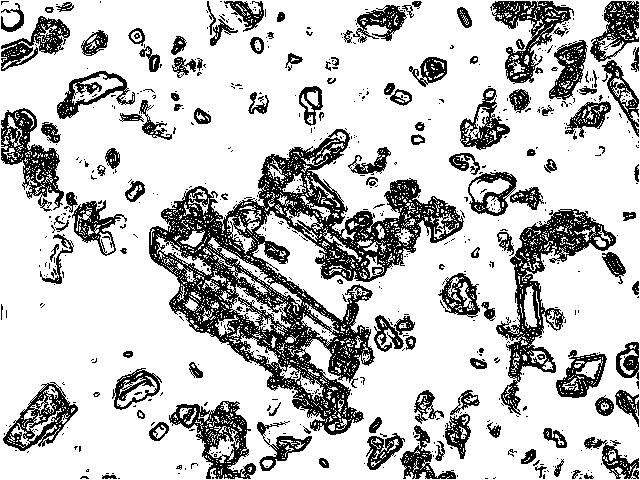
\includegraphics[width=\textwidth]{yen_image}
        \caption{Imagen tras aplicarla segmentación}
    \end{subfigure}
    \caption{Segementación de una imagen}
	\label{fig:3.4.0}
\end{figure}

Posteriormente a este paso, nos interesa, como es obvio, dividir la parte delantera de la imagen resultante en objetos. De este modo, obtendremos cada uno de los objetos por separado de forma idónea.

\subsubsection{Binarización}

La binarización de una imagen consiste en la simplificación de los valores de cada píxel a 2 posibles valores, blanco o negro, representando el fondo y el frente de la imagen cada uno de ellos. Esta técnica nos permite conservar únicamente la información que nos interesa, eliminando el resto.

\subsubsection{Thresholding}

Es el método mas simple para la segmentación de una imagen, pudiendose utilizar para la binarización de una imagen, como es nuestro caso. Consiste en reemplazar los píxeles por debajo de una determinada constante a píxeles negros, y los que se encuentran por encima a píxeles blancos o viceversa. Un ejemplo de una imagen a la que se le ha aplicado esta técnica se muestra en la figura \ref{fig:3.2.1}.

\begin{figure}
\centering
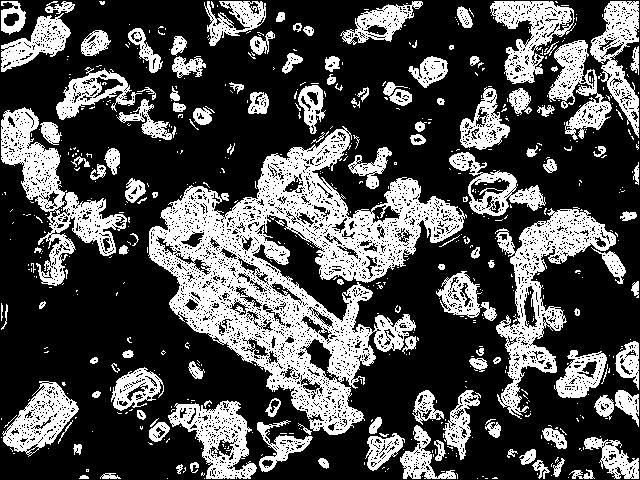
\includegraphics[width=0.5\textwidth]{adaptive_thresholded_image_5}
\caption{Ejemplo de imagen tras aplicar \textit{thresholding}.}
\label{fig:3.2.1}
\end{figure}

Existen distintas maneras de llevar a cabo este proceso, siendo uno de lo más conocidos el método de Otsu~\cite{wiki:otsu}.

\subsection{Descriptores visuales}

Los descriptores visuales, o descriptores de características, son descripciones de las características visuales de los contenidos en imágenes o videos, en nuestro caso de imágenes, con el propósito de la detección de objetos~\cite{wiki:visualdescriptor}. El objetivo de los descriptores visuales es obtener la información que resulta significativa, eliminando a su vez la que no lo es. Así, utilizaremos la información que el descriptor nos proporciona para detectar los objetos que nos interesan en una imagen. Algunos ejemplos de características son la forma, el color o la textura.

Como se puede imaginar, obtener las características a mano es una tarea complicada y que usualmente no funciona correctamente. Por ello, utilizamos un método de extracción automática de características como es \textit{Histogram of Oriented Gradients} (HoG), el cual se basa en los gradientes de la imagen para detectar los distintos objetos que se encuentran en la imagen~\cite{wiki:hog}. En la figura \ref{fig:3.4.2} observamos el resultado de la obtención de las características de HoG de una imagen ejemplo.

\begin{figure}
\centering
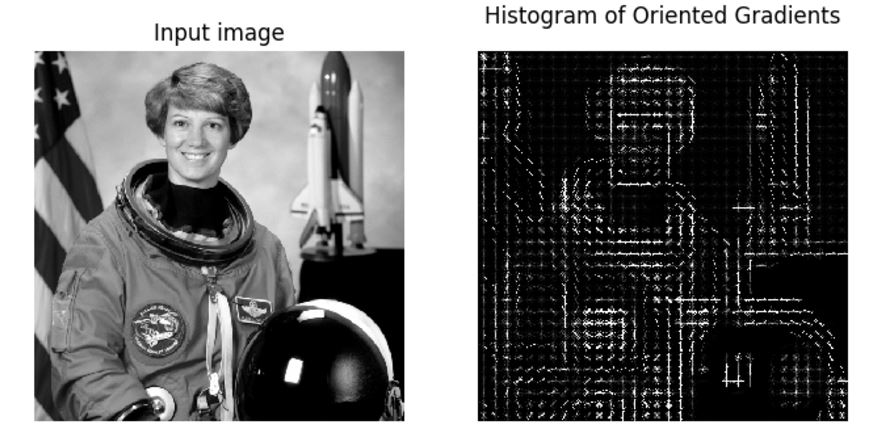
\includegraphics[width=0.8\textwidth]{hog_example}
\caption{Ejemplo de las características de HoG.}
\label{fig:3.4.2}
\end{figure}

\subsection{\textit{Data augmentation}}

\textit{Data augmentation} es una técnica utilizada cuando se posee un conjunto de datos reducido\footnote{En nuestro caso, hacemos referencia a un conjunto pequeño de imágenes.} o incompleto~\cite{emalgorithm}. Permitiéndonos aumentar significativamente nuestro conjunto de datos o completarlo. 

En el caso de la aplicación de esta técnica sobre un conjunto de imágenes, se trata de aplicar distintos filtros y efectos: espejados, rotaciones, ruido, recortes de la imagen, inversiones de colores, oscurecimientos o aclaramientos, difuminaciones, normalizaciones, conversiones a escala de grises, reescalamientos, entre otras. Un posible ejemplo de las imágenes resultantes tras aplicar algunos de los efectos anteriores, y combinándolos entre sí, lo observamos en la figura~\ref{fig:3.4.1}, en la que observamos 64 imágenes resultantes de aplicar efectos sobre una única imagen.

\begin{figure}
\centering
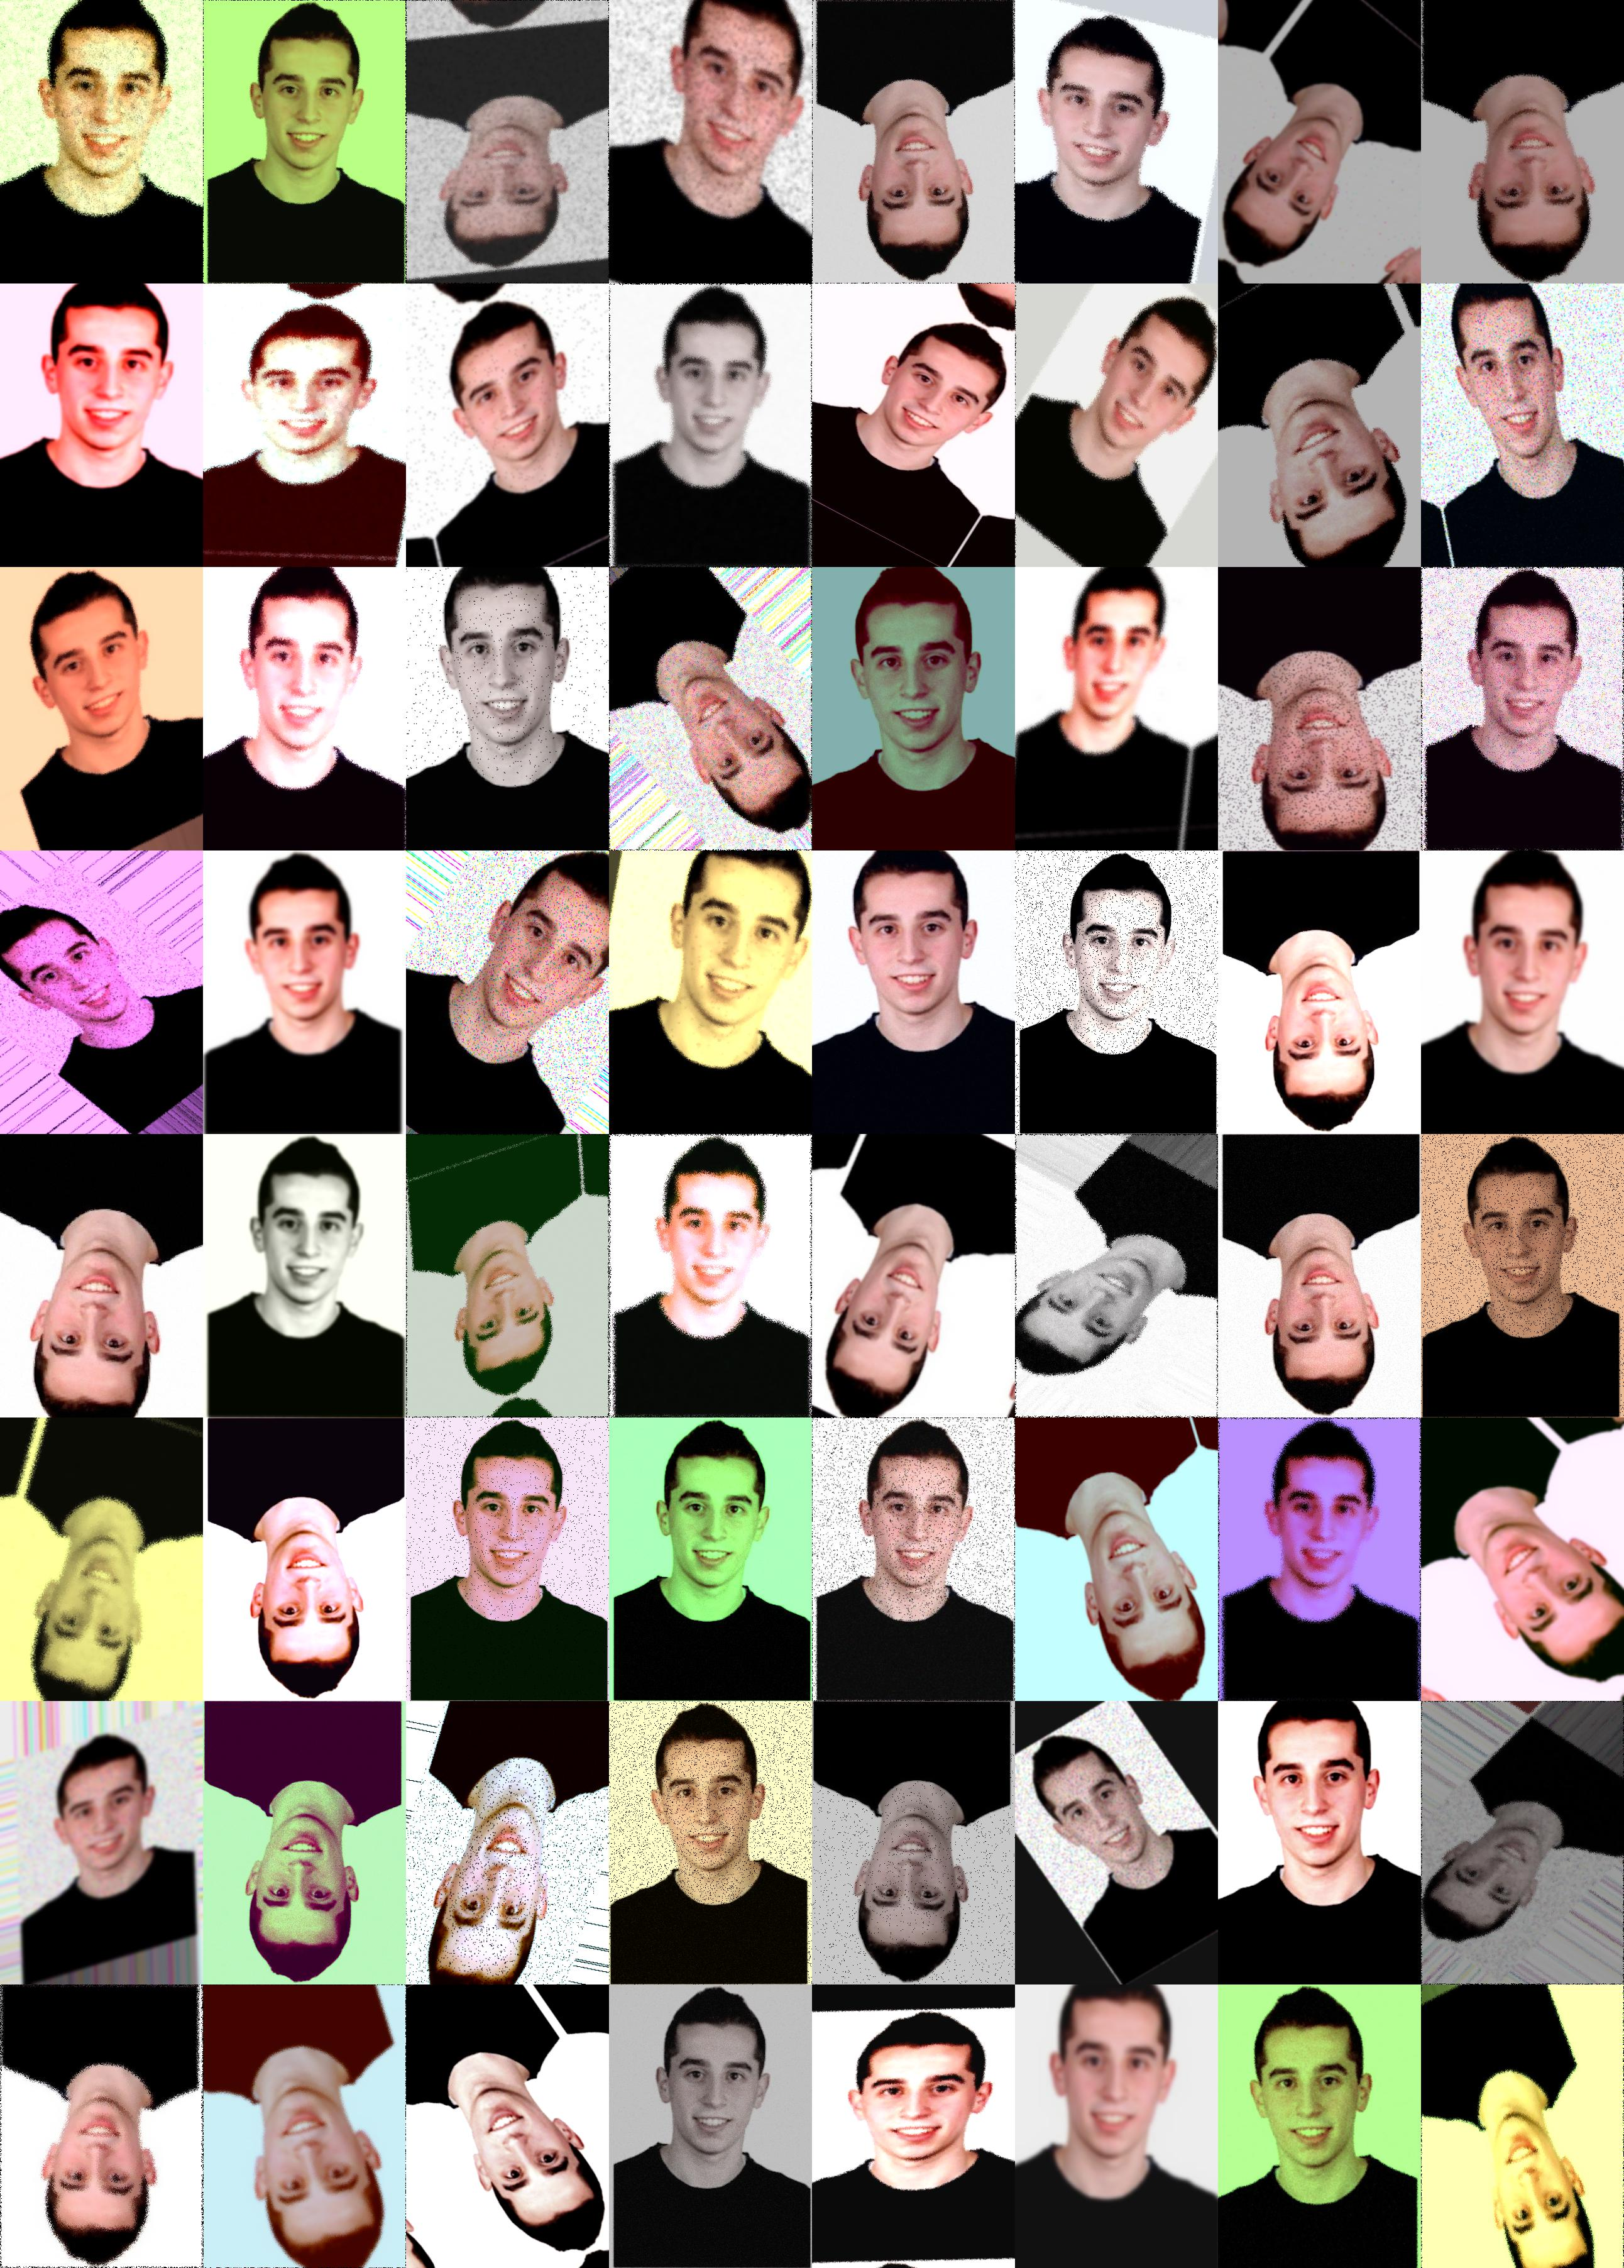
\includegraphics[width=0.8\textwidth]{DataAugmentationExample}
\caption{Ejemplo de \textit{data augmentation.}}
\label{fig:3.4.1}
\end{figure}

\section{Detección de objetos}

\subsection{Reconocimiento de objetos contra Detección de objetos}

Antes de abordar el siguiente concepto, debemos de comprender la diferencia entre el término reconocimiento de objetos y detección de objetos.

Reconocimiento de objetos es el término utilizado cuando se desea detectar todos los objetos para los que ha sido entrenado el clasificador. Proporcionándonos el tipo de objeto y las coordenadas de la caja que rodea ese objeto. Dependiendo del algoritmo de clasificación empleado, también puede devolver las probabilidades de que ese objeto sea un verdadero positivo o un falso positivo.

En cuanto a la detección de objetos, en este solo se desea obtener si es objeto o no. Simplificando el problema anterior, de manera que, pasamos de un problema multiclase a un problema con dos clases, o binario: Objeto o no objeto.

%\section{VOC}?

%\section{Redes neuronales y redes neuronales convolucionales}

\section{Aprendizaje profundo}

Aprendizaje profundo, o más comunmente mencionado en inglés mediante las palabras \textit{deep learning}, es la técnica más avanzada, catalogada como el estado del arte, para ámbitos como la visión artificial, el reconocimiento de voz automático, el procesamiento del lenguaje natural,  la bioinformática y el reconocimiento de audio, entre otros campos~\cite{ms:deeplearning}.

\textit{Deep learning} es un conjunto de algoritmos de la rama del aprendizaje automático que se caracteriza por los siguientes aspectos, principalmente~\cite{ms:deeplearning}:

\begin{enumerate}
	\item Consisten en modelos con varias capas en las que la información sufre a menudo operaciones no lineales.
	\item Consisten en representaciones de características que parten desde un nivel bajo de abstracción hasta llegar a un nivel alto. Por ejemplo, desde los píxeles de la imagen hasta las clases de objetos y sus coordenadas dentro de la imagen.
\end{enumerate}

Este conjunto de técnicas es la intersección entre las redes neuronales, la inteligencia artificial, el modelado de grafos, la optimización, el reconocimiento de patrones y el procesado de señales~\cite{ms:deeplearning}. % Aclarar algunos de los conceptos

Pero no todo son ventajas en esta aproximación. Y es que existe un problema principal: el cual es el volumen de imágenes que necesita un modelo de este tipo para ser adecuadamente entrenado, del orden de miles o cientos de miles. Por otro lado, el tiempo necesario para entrenar un modelo de este tipo es enorme, sino se posee una tarjeta gráfica especialmente potente. Y, por último, estos son modelos de caja negra, es decir, que difícilmente resultan comprensibles para un ser humano. Más adelante indagaremos en posibles soluciones.

\subsection{\textit{YOLO}}

\textit{YOLO}, o \textit{You Only Look Once}~\cite{yolo}, es una aproximación innovadora en la detección de objetos, considerado actualmente, como el estado del arte en esta materia, junto a \textit{Faster RCNN}~\cite{faster-rcnn}\footnote{Faster RCNN es un detector de objetos en tiempo real con una precisión similar a la última versión de \textit{YOLO}, pero con menor rendimiento en tiempos que \textit{este}.}. Tratando de crear una arquitectura que funciona en tiempo real pero, a su vez, siendo capaz de soportar un número de clases mayor a 9000~\cite{yolov2}.

\subsubsection{Versiones}

\textit{YOLO} actualmente tiene dos versiones. Y, en cada una de estas versiones, se ha desarrollado una versión pequeña y una normal. En la primera versión de \textit{YOLO} se consiguió llegar a resultados muy positivos, como la capacidad de procesar 45 imágenes por segundo con una precisión de 63.4 \textit{mAP}\footnote{\textit{Mean average precision} (mAP), o Media promedio de precisión, es comúnmente utilizada como una medida de evaluación de la precisión en la detección de objetos.}. Y, con la versión pequeña de este, se llegaron a procesar 155 imágenes por segundo con una precisión de 52.7 \textit{mAP}~\cite{yolo}. Precisiones muy positivas, pero que todavía no estaban a la altura del estado del arte a nivel de precisión.

En la segunda versión, se considera a \textit{YOLO} como el estado del arte, junto a \textit{Faster RCNN}. En esta versión, \textit{YOLO} consigue llegar a una precisión de 76,8 \textit{mAP}, procesando 67 imágenes por segundo, y 78,6 \textit{mAP}, procesando 40 imágenes por segundo. Lo cual, supera a \textit{Faster RCNN} en precisión y rapidez, siendo esta última ampliamente superada~\cite{yolov2}.\footnote{\textit{Faster RCNN} consigue clasificar una imagen cada dos segundos(\textit{FPS, frames per second}). En cambio, \textit{YOLO} es capaz de procesar más de 40 imágenes.}

\subsubsection{Característica diferenciadora de \textit{YOLO}}

\textit{YOLO} otorga un enfoque distinto respecto a sus competidores. Mientras que en otros casos, como \textit{Faster RCNN}, se separan las distintas etapas del procesado de una imagen. \textit{YOLO}, he de aquí su nombre, solo necesita de un único <<vistazo>> para predecir la imagen y obtener las coordenadas, o cajas que rodean a cada uno de los objetos predichos~\cite{yolo}. Véase la figura \ref{fig:3.2.14}.

\begin{figure}[h]
\centering
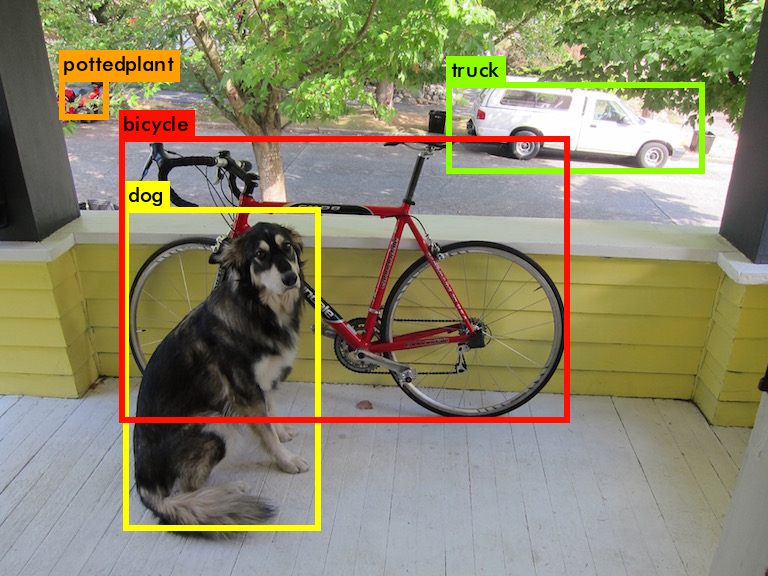
\includegraphics[width=0.6\textwidth]{yolo_example}
\caption{Imagen predicha por \textit{YOLO}}
\label{fig:3.2.14}
\end{figure}

Por supuesto, esta perspectiva no es tan simple como un giro en el enfoque. Sino que, además, implementa otras características, como la normalización en lotes o la obtención automática del tamaño de las cajas, que la permiten ser la mejor aproximación actual en este campo~\cite{yolov2}.

Podemos ver una comparativa entre los mejores detectores de objetos actuales con \textit{YOLO} en la tabla \ref{tabla:comparativa_yolo}. Indicando para cada uno de ellos la precisión y la capacidad de procesamiento de imágenes, en las unidades de media promedio de precisión e imágenes por segundo, respectivamente.

\begin{table}
  \begin{center}
  \caption[Comparativa entre los distintos sistemas de detección de objetos]{Comparativa entre los distintos sistemas de detección de objetos sobre el mismo conjunto de entrenamiento y sobre la misma configuración~\cite{yolov2}.}
    \label{tabla:comparativa_yolo}
    \begin{tabular}{@{} l l r r@{}}
      \toprule
        \textbf{Detection frameworks}  & \textbf{Train} & \textbf{$mAP$} & \textbf{FPS} \\
      \midrule
        Fast R-CNN                     & 2007+2012      & 70.0           & 0.5 \\
        Faster R-CNN VGG-16                            & 2007+2012      & 73.2           & 7 \\
      Faster R-CNN Resnet                            & 2007+2012      & 76.4           & 5 \\
      YOLO                            & 2007+2012      & 63.4          & 45 \\
      SDD300                            & 2007+2012      & 74.3           & 46 \\
      SDD500                            & 2007+2012      & 76.8           & 19 \\\hline
      YOLOv2 288 x 288                            & 2007+2012      & 69           & 91 \\
      YOLOv2 352 x 352                            & 2007+2012      & 73.7           & 81 \\
      YOLOv2 416 x 416                            & 2007+2012      & 76.8           & 67 \\
      YOLOv2 480 x 480                            & 2007+2012      & 77.8           & 59 \\
      YOLOv2 544 x 544                            & 2007+2012      & 78.6           & 40 \\
      \bottomrule
    \end{tabular}
  \end{center}
\end{table}


% Por aclarar más cosas